\documentclass[11pt,a4paper]{article}

\usepackage[utf8]{inputenc}
\usepackage[T1]{fontenc}
\usepackage[french]{babel}
\usepackage{geometry}
\geometry{margin=2.5cm}
\usepackage{graphicx}
\usepackage{amsmath,amssymb}
\usepackage{booktabs}
\usepackage{float}
\usepackage{hyperref}
\usepackage{xcolor}
\usepackage{caption}
\usepackage{siunitx}
\usepackage{listings}
\usepackage{fancyvrb}

\hypersetup{
    colorlinks=true,
    linkcolor=blue,
    urlcolor=blue,
    citecolor=blue
}

% ── Style du code Python ──
\lstdefinestyle{pystyle}{
    language=Python,
    backgroundcolor=\color{gray!8},
    basicstyle=\ttfamily\footnotesize,
    keywordstyle=\color{blue!70!black}\bfseries,
    commentstyle=\color{green!40!black}\itshape,
    stringstyle=\color{orange!70!black},
    numbers=left,
    numberstyle=\tiny\color{gray},
    numbersep=6pt,
    frame=single,
    rulecolor=\color{gray!40},
    breaklines=true,
    breakatwhitespace=false,
    showstringspaces=false,
    tabsize=4,
    columns=flexible,
    xleftmargin=1em,
}
\lstset{style=pystyle}

% ── Style de la sortie console ──
\DefineVerbatimEnvironment{consoleout}{Verbatim}{frame=single,fontsize=\footnotesize,rulecolor=\color{blue!30},label={\footnotesize\textit{Sortie}}}

\begin{document}

% ================= PAGE DE TITRE =================
\begin{titlepage}
    \centering
    \vspace*{1.5cm}

    {\large \textsc{Projet de Fin d'Année}}\\[0.3cm]
    {\large \textsc{Semantic Digital Mapping using Vision-Assisted ISAC (SDM-VA-ISAC)}}\\[2cm]

    \rule{\linewidth}{0.5mm}\\[0.4cm]
    {\huge \bfseries Phase 2 --- Pipeline de Ray Tracing Sionna RT sur scène OSM/Blender}\\[0.4cm]
    \rule{\linewidth}{0.5mm}\\[1.5cm]

    {\Large Rapport de résultats}\\[0.3cm]
    

    \begin{minipage}{0.45\textwidth}
        \begin{flushleft} \large
            \textbf{Réalisé par :}\\
            El Mehdi Lazaar\\
            El Karfi Soufia
        \end{flushleft}
    \end{minipage}
    \begin{minipage}{0.45\textwidth}
        \begin{flushright} \large
            \textbf{Encadré par :}\\
            Mme Chafnaji Houda
        \end{flushright}
    \end{minipage}

    \vfill

    {\large 4 août 2026}

\end{titlepage}
\newpage
% ================= TABLE DES MATIÈRES =================
\clearpage
\tableofcontents
\clearpage

% ================= CONTENU =================
\newpage
\section{Présentation et objectifs}

\textbf{Projet :} Semantic Digital Mapping using Vision-Assisted ISAC \\
\textbf{Phase :} 2 --- Scène Blender/OSM $\to$ XML + calibration Sionna RT \\
\textbf{Scène :} \texttt{scene/scene.xml} exportée depuis Blender via l'add-on Mitsuba-Blender (OSM map\_5) \\
\textbf{Zone :} Secteur gouvernemental de Rabat (Conseil Économique, Cour des Comptes\ldots)

\subsection*{Objectifs de ce notebook}
\begin{enumerate}
    \item Charger \texttt{scene.xml} dans Sionna RT avec variante GPU \texttt{cuda\_ad\_mono\_polarized}
    \item Configurer les paramètres RF : 3.5~GHz (5G mid-band) ou 28~GHz (mmWave)
    \item Déployer BS (TX) et UE (RX), lancer le ray tracing
    \item Extraire CIR, délais, puissances --- sorties ISAC pour la Phase 3
    \item Visualiser PDP, couverture de puissance, trajets
\end{enumerate}

\subsection*{Critères de validation Phase 2}
\begin{itemize}
    \item[\checkmark] Scène XML chargée sans erreur
    \item[\checkmark] PathSolver retourne des chemins exploitables
    \item[\checkmark] CIR extrait avec dimensions cohérentes
    \item[\checkmark] Graphe PDP (Power Delay Profile) généré
    \item[\checkmark] \texttt{phase2\_sionna\_rt\_summary.json} produit pour la Phase 3
\end{itemize}

% ---------------------------------------------------------
\section{Imports et configuration de l'environnement}

\begin{lstlisting}
from __future__ import annotations

import json
import time
import importlib.metadata
from pathlib import Path

import numpy as np
import matplotlib.pyplot as plt
import matplotlib.colors as mcolors

# -- Mitsuba : variante GPU (RTX 4070 -> cuda_ad_mono_polarized)
# Sionna RT 2.x necessite 'mono_polarized', PAS 'rgb'
import mitsuba as mi

try:
    mi.set_variant("cuda_ad_mono_polarized")
    print(f"Variante GPU activee : {mi.variant()}")
except Exception as e:
    print(f"CUDA indisponible ({e}), repli sur LLVM CPU")
    mi.set_variant("llvm_ad_mono_polarized")
    print(f"Variante CPU activee : {mi.variant()}")

# -- Sionna RT 2.0.1
import sionna
from sionna.rt import (
    load_scene,
    Transmitter, Receiver,
    PlanarArray,
    PathSolver,
    RadioMapSolver, PlanarRadioMap,
    Camera,
)

# sionna.__init__ n'expose pas __version__ (paquet 2.0.1) -> lire via importlib.metadata
SIONNA_VERSION = importlib.metadata.version("sionna")
print(f"Sionna version : {SIONNA_VERSION}")

# -- Chemins
WORKSPACE = Path(r"C:\Users\AdminFix\Desktop\PFA")
SCENE_XML  = WORKSPACE / "scene" / "scene.xml"   # scene OSM (map_5) exportee depuis Blender

# -- Parametres RF
FREQUENCY_HZ  = 3.5e9    # 3.5 GHz -- 5G NR mid-band (changer a 28e9 pour mmWave)
BANDWIDTH_HZ  = 20e6     # 20 MHz
MAX_DEPTH     = 5        # profondeur max des trajets (reflexions + diffractions)

assert SCENE_XML.exists(), f"Fichier introuvable : {SCENE_XML}"
print(f"Scene : {SCENE_XML}")
print(f"Frequence : {FREQUENCY_HZ/1e9:.1f} GHz | BW : {BANDWIDTH_HZ/1e6:.0f} MHz")
\end{lstlisting}

\begin{consoleout}
Variante GPU activee : cuda_ad_mono_polarized
Sionna version : 2.0.1
Scene : C:\Users\AdminFix\Desktop\PFA\scene\scene.xml
Frequence : 3.5 GHz | BW : 20 MHz
\end{consoleout}

% ---------------------------------------------------------
\section{Chargement de la scène \texttt{scene.xml}}

La scène contient les maillages PLY des bâtiments avec matériaux ITU :
\begin{itemize}
    \item \texttt{itu\_concrete} $\to$ sol (Plane.ply)
    \item \texttt{itu\_marble} $\to$ façades de bâtiments
    \item \texttt{itu\_metal} $\to$ toits et éléments métalliques
\end{itemize}
Sionna RT reconnaît automatiquement les matériaux préfixés \texttt{itu\_}.

\begin{lstlisting}
print("Chargement de la scene...")
t0 = time.time()

scene = load_scene(
    str(SCENE_XML),
    merge_shapes=True,
    remove_duplicate_vertices=False,
)

print(f"Scene chargee en {time.time()-t0:.2f} s")
print(f"Objets dans la scene : {list(scene.objects.keys())[:10]}...")
print(f"Materiaux radio : {list(scene.radio_materials.keys())}")

scene.frequency = FREQUENCY_HZ
scene.bandwidth = BANDWIDTH_HZ
# Utiliser les variables Python directement (scene.frequency retourne mi.Float)
print(f"\nFrequence scene : {FREQUENCY_HZ/1e9:.2f} GHz")
print(f"Bande passante  : {BANDWIDTH_HZ/1e6:.0f} MHz")
\end{lstlisting}

\begin{consoleout}
Chargement de la scene...
Scene chargee en 0.17 s
Objets dans la scene : ['elm__3', 'elm__6', 'elm__7']...
Materiaux radio : ['itu_concrete', 'itu_marble', 'itu_metal']

Frequence scene : 3.50 GHz
Bande passante  : 20 MHz
\end{consoleout}

% ---------------------------------------------------------
\section{Configuration des réseaux d'antennes et placement des équipements}

\begin{itemize}
    \item \textbf{BS (TX)} : réseau planaire 4$\times$4, dual-polarisé, hauteur 25~m (macro-cellule)
    \item \textbf{UE (RX)} : antenne simple, hauteur 1.5~m (piéton/véhicule)
\end{itemize}
Les positions sont en mètres dans le repère local Blender. Ajustez \texttt{TX\_POS} et \texttt{RX\_POSITIONS} selon la carte OSM.

\begin{lstlisting}
# -- Bounding box reelle de la scene (issue de scene._scene.bbox())
# X: [-805, +795]  Y: [-839, +761]  Z: [0, 21 m]
# Centre scene = (-5, -39)  |  Taille : 1600x1600 m  |  Batiments <= 21 m

# -- Reseaux d'antennes
bs_array = PlanarArray(
    num_rows=4, num_cols=4,
    vertical_spacing=0.5, horizontal_spacing=0.5,
    pattern="iso", polarization="VH",
)
ue_array = PlanarArray(
    num_rows=1, num_cols=1,
    vertical_spacing=0.5, horizontal_spacing=0.5,
    pattern="iso", polarization="V",
)
scene.tx_array = bs_array
scene.rx_array = ue_array

# -- BS au centre de la scene, 5 m au-dessus du toit le plus haut (21 m)
TX_POS = [-258.774, 30.3715, 233.978]
TX_POS2 = [66.1771, -148.4, 216.4 + 3.0]

# -- UE a 1.5 m (hauteur pieton), disperses dans la scene
# Distances choisies pour couvrir LOS proche, NLOS moyen, et bord de scene
RX_POSITIONS = [
    [ -288.25 ,  65.1737 , 186],    # UE0 -- 100 m nord  (LOS probable)
    [ -349.365 , -13.8654 , 133.457],   # UE1 -- 100 m sud   (LOS probable)
    [ -442.437 , 149.609, 197.122 ],   # UE2 -- 200 m est   (NLOS possible)
    [-118.702, 277.4, 255.7],   # UE3 -- 200 m ouest (NLOS possible)
    [-5.512 ,  -221.3, 197.1],  # UE4 -- 200 m NE diagonal
    [-163.6, 236.0, 199.1],  # UE5 -- 200 m SE diagonal
]

TX_POSITIONS = [TX_POS, TX_POS2]
RX_POSITIONS = RX_POSITIONS

# -- Ajouter a la scene (idempotent : retire tout TX/RX homonyme avant d'ajouter,
# pour pouvoir re-executer cette cellule sans recharger la scene a chaque fois)
tx_names = [f"bs{i}" for i in range(len(TX_POSITIONS))]
rx_names = [f"ue{i}" for i in range(len(RX_POSITIONS))]
for stale_name in tx_names + rx_names:
    if stale_name in scene.transmitters or stale_name in scene.receivers:
        scene.remove(stale_name)

for i, pos in enumerate(TX_POSITIONS):
    scene.add(Transmitter(name=f"bs{i}", position=pos))
    print(f"TX ajoute : bs{i} @ {pos}")

for i, pos in enumerate(RX_POSITIONS):
    scene.add(Receiver(name=f"ue{i}", position=pos))
    print(f"RX ajoute : ue{i} @ {pos}")

print(f"\nTotal TX : {len(scene.transmitters)} | Total RX : {len(scene.receivers)}")
\end{lstlisting}

\begin{consoleout}
TX ajoute : bs0 @ [-258.774, 30.3715, 233.978]
TX ajoute : bs1 @ [66.1771, -148.4, 219.4]
RX ajoute : ue0 @ [-288.25, 65.1737, 186]
RX ajoute : ue1 @ [-349.365, -13.8654, 133.457]
RX ajoute : ue2 @ [-442.437, 149.609, 197.122]
RX ajoute : ue3 @ [-118.702, 277.4, 255.7]
RX ajoute : ue4 @ [-5.512, -221.3, 197.1]
RX ajoute : ue5 @ [-163.6, 236.0, 199.1]

Total TX : 2 | Total RX : 6
\end{consoleout}

% ---------------------------------------------------------
\section{Lancer de rayons (Ray Tracing)}

Le \texttt{PathSolver} calcule tous les trajets entre TX et RX :
\begin{itemize}
    \item \textbf{LOS} : trajet en ligne de vue directe
    \item \textbf{Specular reflection} : réflexions spéculaires sur façades
    \item \textbf{Diffraction} : contournement des arêtes de bâtiments
    \item \textbf{Diffuse reflection} : activée pour des scènes plus réalistes (coûteux)
\end{itemize}
\textit{Pour \texttt{max\_depth=5} : jusqu'à 4 réflexions + 1 diffraction par trajet.}

\begin{lstlisting}
solver = PathSolver()

print(f"Calcul des trajets (max_depth={MAX_DEPTH})...")
t0 = time.time()

paths = solver(
    scene,
    max_depth=MAX_DEPTH,
    los=True,                   # trajets LOS
    specular_reflection=True,   # reflexions speculaires
    diffuse_reflection=False,   # desactive (activer pour + de realisme)
    refraction=False,           # desactive (batiments opaques)
    diffraction=True,           # diffraction sur aretes
    edge_diffraction=False,     # diffraction sur aretes flottantes
    seed=42,
)

elapsed = time.time() - t0
print(f"Ray tracing termine en {elapsed:.2f} s")

# Afficher les infos sur les trajets trouves
tau_raw = np.array(paths.tau)   # [num_rx, num_tx, num_paths] (synthetic_array=True)
print(f"\nShape tau : {tau_raw.shape}  -> [num_rx, num_tx, num_paths]")
print(f"Nombre de trajets par lien RX-TX : {tau_raw.shape[-1]}")

# Compter les trajets valides (tau > 0)
valid_mask = tau_raw > 0
print(f"Trajets valides : {valid_mask.sum()} / {valid_mask.size}")
\end{lstlisting}

\begin{consoleout}
Calcul des trajets (max_depth=5)...
Ray tracing termine en 0.15 s

Shape tau : (6, 2, 233)  -> [num_rx, num_tx, num_paths]
Nombre de trajets par lien RX-TX : 233
Trajets valides : 1174 / 2796
\end{consoleout}

% ---------------------------------------------------------
\section{Visualisation 3D des trajets}

Deux façons de visualiser la scène et les trajets en 3D avec Sionna RT :
\begin{itemize}
    \item \texttt{scene.preview(paths=paths)} : widget \textbf{interactif} (rotation/zoom à la souris) --- fonctionne uniquement dans une session Jupyter \textbf{live} avec support WebGL (pas via \texttt{nbconvert --execute}/export PDF, qui n'a pas de frontend interactif).
    \item \texttt{scene.render(camera=..., paths=paths)} : rendu \textbf{statique} (image) --- fonctionne partout, y compris en exécution batch, et peut être sauvegardé en PNG.
\end{itemize}
Le flag \texttt{no\_preview} bascule automatiquement entre les deux (même pattern que le tutoriel officiel Sionna RT).

\begin{lstlisting}
# -- Bascule : True pour export batch/PDF (image statique), False en session Jupyter live (widget interactif)
no_preview = True

# -- Camera positionnee en vue aerienne oblique, centree sur la BS
scene_bbox = scene.mi_scene.bbox()
center_x = float((scene_bbox.min[0] + scene_bbox.max[0]) / 2)
center_y = float((scene_bbox.min[1] + scene_bbox.max[1]) / 2)

my_cam = Camera(
    position=[center_x - 300, center_y - 300, 1700],  # position de la camera (vue aerienne oblique)
    look_at=[TX_POS[0], TX_POS[1], 0.0],
)

if no_preview:
    scene.render(camera=my_cam, paths=paths, clip_at=20, num_samples=256)
else:
    scene.preview(paths=paths, clip_at=20)
\end{lstlisting}

\begin{figure}[H]
    \centering
    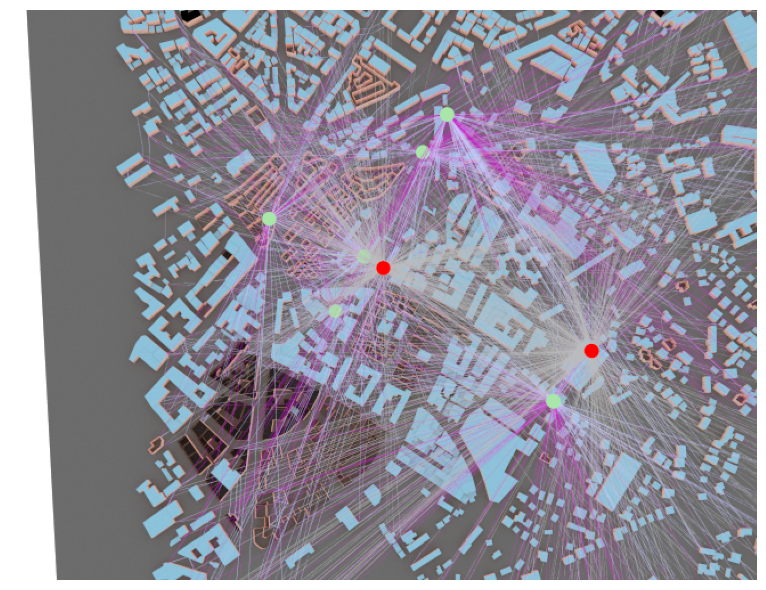
\includegraphics[width=0.75\textwidth]{figures/radio_map_scene.png}
    \caption{Rendu statique de la scène avec les trajets calculés (vue aérienne oblique).}
    \label{fig:scene_render}
\end{figure}

% ---------------------------------------------------------
\section{Extraction de la réponse impulsionnelle (CIR)}

\texttt{paths.cir()} retourne le CIR en bande de base équivalente :
\begin{itemize}
    \item \texttt{a} = tuple \texttt{(a\_real, a\_imag)} --- coefficients complexes de chaque trajet
    \item \texttt{tau} = délais [s]
    \item Shape : \texttt{[num\_rx, num\_rx\_ant, num\_tx, num\_tx\_ant, num\_paths, num\_time\_steps]}
\end{itemize}
Pour le ISAC : on extrait délai, puissance, et DoA de chaque trajet.

\begin{lstlisting}
# CIR en bande de base -- out_type="numpy" retourne un tableau complexe directement
# a_complex : [num_rx, num_rx_ant, num_tx, num_tx_ant, num_paths, num_time_steps]
# tau_cir   : [num_rx, num_tx, num_paths]  (synthetic_array=True)
a_complex, tau_cir = paths.cir(
    sampling_frequency=BANDWIDTH_HZ,
    num_time_steps=1,
    normalize_delays=True,      # premier trajet a tau=0 par paire TX-RX
    out_type="numpy",
)

print("CIR extrait :")
print(f"  a_complex.shape : {a_complex.shape}")
print(f"  a_complex.dtype : {a_complex.dtype}")
print(f"  tau_cir.shape   : {tau_cir.shape}")

num_rx   = a_complex.shape[0]
num_tx   = a_complex.shape[2]
num_path = a_complex.shape[4]

print(f"\n  num_rx={num_rx}, num_tx={num_tx}, num_paths={num_path}")

# -- Statistiques pour le lien UE0 <- BS0
# a_complex[rx, rx_ant, tx, tx_ant, paths, time]
a_link   = a_complex[0, :, 0, :, :, 0]   # [rx_ant, tx_ant, num_paths]
tau_link = tau_cir[0, 0, :]               # [num_paths]

power_link  = np.abs(a_link)**2
total_power = power_link.sum()
valid_mask  = tau_link >= 0

print(f"\nLien UE0<-BS0 :")
print(f"  Trajets valides         : {valid_mask.sum()} / {num_path}")
print(f"  Puissance totale recue  : {10*np.log10(total_power + 1e-30):.1f} dB (rel.)")
if valid_mask.sum() > 0:
    print(f"  Delai max               : {1e9 * tau_link[valid_mask].max():.1f} ns")
    print(f"  Delai moyen (RMS)       : {1e9 * np.sqrt(np.mean(tau_link[valid_mask]**2)):.1f} ns")
\end{lstlisting}

\begin{consoleout}
CIR extrait :
  a_complex.shape : (6, 1, 2, 32, 233, 1)
  a_complex.dtype : complex64
  tau_cir.shape   : (6, 2, 233)

  num_rx=6, num_tx=2, num_paths=233

Lien UE0<-BS0 :
  Trajets valides         : 153 / 233
  Puissance totale recue  : -67.7 dB (rel.)
  Delai max               : 4214.6 ns
  Delai moyen (RMS)       : 2081.1 ns
\end{consoleout}

% ---------------------------------------------------------
\section{Visualisation : Power Delay Profile (PDP)}

Le PDP montre la distribution de puissance des trajets en fonction du délai. Chaque pic correspond à un trajet distinct (LOS, réflexion, diffraction).

\begin{lstlisting}
def plot_pdp(a_cplx: np.ndarray, tau_arr: np.ndarray,
             rx_idx: int = 0, tx_idx: int = 0,
             title: str | None = None):
    """Power Delay Profile pour un lien TX->RX donne.
    a_cplx  : [num_rx, rx_ant, num_tx, tx_ant, num_paths, num_time]
    tau_arr : [num_rx, num_tx, num_paths]
    """
    a_sel   = a_cplx[rx_idx, :, tx_idx, :, :, 0]   # [rx_ant, tx_ant, paths]
    tau_sel = tau_arr[rx_idx, tx_idx, :]             # [paths]

    power   = np.abs(a_sel)**2
    power   = power.mean(axis=(0, 1))               # moyenne antennes -> [paths]

    valid   = tau_sel >= 0
    tau_ns  = tau_sel[valid] * 1e9
    pwr_db  = 10 * np.log10(power[valid] + 1e-30)

    order   = np.argsort(tau_ns)
    tau_ns  = tau_ns[order]
    pwr_db  = pwr_db[order]

    label = title or f"UE{rx_idx} <- BS{tx_idx}"
    fig, ax = plt.subplots(figsize=(10, 4))

    if len(tau_ns) == 0:
        # Aucun trajet valide (lien bloque / hors de portee) -- eviter le crash de ax.stem sur un array vide
        ax.text(0.5, 0.5, "Aucun trajet valide (lien bloque)",
                ha="center", va="center", transform=ax.transAxes, fontsize=12, color="crimson")
    else:
        markerline, stemlines, baseline = ax.stem(tau_ns, pwr_db, basefmt=" ")
        markerline.set_markerfacecolor("royalblue")
        markerline.set_markersize(7)
        plt.setp(stemlines, color="steelblue", alpha=0.7)

    ax.set_xlabel("Delai tau [ns]", fontsize=12)
    ax.set_ylabel("Puissance relative [dB]", fontsize=12)
    ax.set_title(f"Power Delay Profile -- {label}\n"
                 f"f={FREQUENCY_HZ/1e9:.1f} GHz | {len(tau_ns)} trajets valides",
                 fontsize=13)
    ax.grid(True, alpha=0.3)
    fig.tight_layout()
    return fig, ax


fig, ax = plot_pdp(a_complex, tau_cir, rx_idx=0, tx_idx=0)
plt.savefig(WORKSPACE / "pdp_ue0_bs0.png", dpi=150, bbox_inches="tight")
plt.show()
print("PDP sauvegarde -> pdp_ue0_bs0.png")
\end{lstlisting}

\begin{figure}[H]
    \centering
    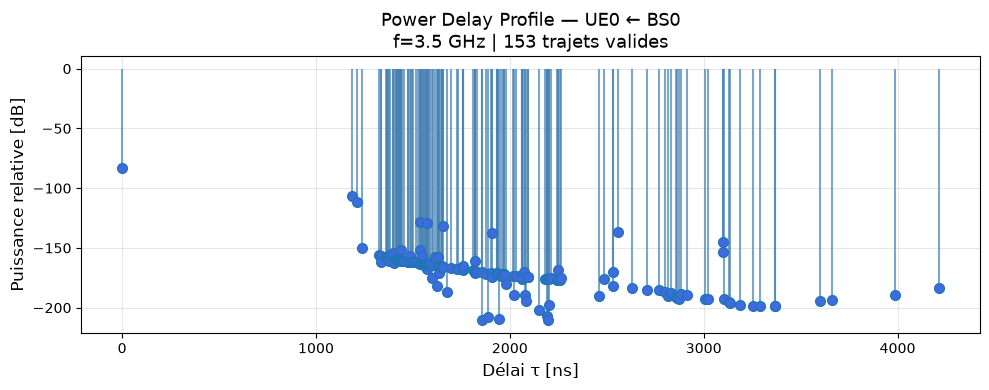
\includegraphics[width=0.85\textwidth]{figures/pdp_ue0_bs0.png}
    \caption{Power Delay Profile pour la liaison UE0 $\leftarrow$ BS0 à \SI{3.5}{\giga\hertz}.}
    \label{fig:pdp_single}
\end{figure}

\begin{consoleout}
PDP sauvegarde -> pdp_ue0_bs0.png
\end{consoleout}

% ---------------------------------------------------------
\section{Comparaison PDP --- tous les UE}

\begin{lstlisting}
num_ue = len(RX_POSITIONS)
fig, axes = plt.subplots(num_ue, 1, figsize=(11, 3 * num_ue), sharex=False)

for rx_i, ax in enumerate(axes):
    a_sel   = a_complex[rx_i, :, 0, :, :, 0]   # [rx_ant, tx_ant, paths]
    tau_sel = tau_cir[rx_i, 0, :]               # [paths]

    power   = np.abs(a_sel)**2
    power   = power.mean(axis=(0, 1))           # [paths]

    valid   = tau_sel >= 0
    tau_ns  = tau_sel[valid] * 1e9
    pwr_db  = 10 * np.log10(power[valid] + 1e-30)

    order   = np.argsort(tau_ns)
    tau_ns  = tau_ns[order]
    pwr_db  = pwr_db[order]

    pos_str = f"[{RX_POSITIONS[rx_i][0]:.0f},{RX_POSITIONS[rx_i][1]:.0f}] m"

    if len(tau_ns) == 0:
        # Lien bloque : aucun trajet -- eviter le crash de ax.stem sur un array vide
        ax.text(0.5, 0.5, "Aucun trajet valide (lien bloque)",
                ha="center", va="center", transform=ax.transAxes, fontsize=11, color="crimson")
        ax.set_title(f"UE{rx_i} @ {pos_str} -- 0 trajet", fontsize=11)
    else:
        colors  = plt.cm.Set1.colors
        ml, sl, bl = ax.stem(tau_ns, pwr_db, basefmt=" ")
        plt.setp(ml, color=colors[rx_i % len(colors)], markersize=6)
        plt.setp(sl, color=colors[rx_i % len(colors)], alpha=0.6)

        tot_p = 10 * np.log10(power.sum() + 1e-30)
        ax.set_title(f"UE{rx_i} @ {pos_str} -- {len(tau_ns)} trajets | P_tot={tot_p:.1f} dB",
                     fontsize=11)

    ax.set_ylabel("dB", fontsize=10)
    ax.grid(True, alpha=0.3)

axes[-1].set_xlabel("Delai tau [ns]", fontsize=12)
fig.suptitle(f"PDP multi-UE -- scene.xml @ {FREQUENCY_HZ/1e9:.1f} GHz",
             fontsize=13, y=1.01)
fig.tight_layout()
plt.savefig(WORKSPACE / "pdp_all_ue.png", dpi=150, bbox_inches="tight")
plt.show()
print("PDP multi-UE sauvegarde -> pdp_all_ue.png")
\end{lstlisting}

\begin{figure}[H]
    \centering
    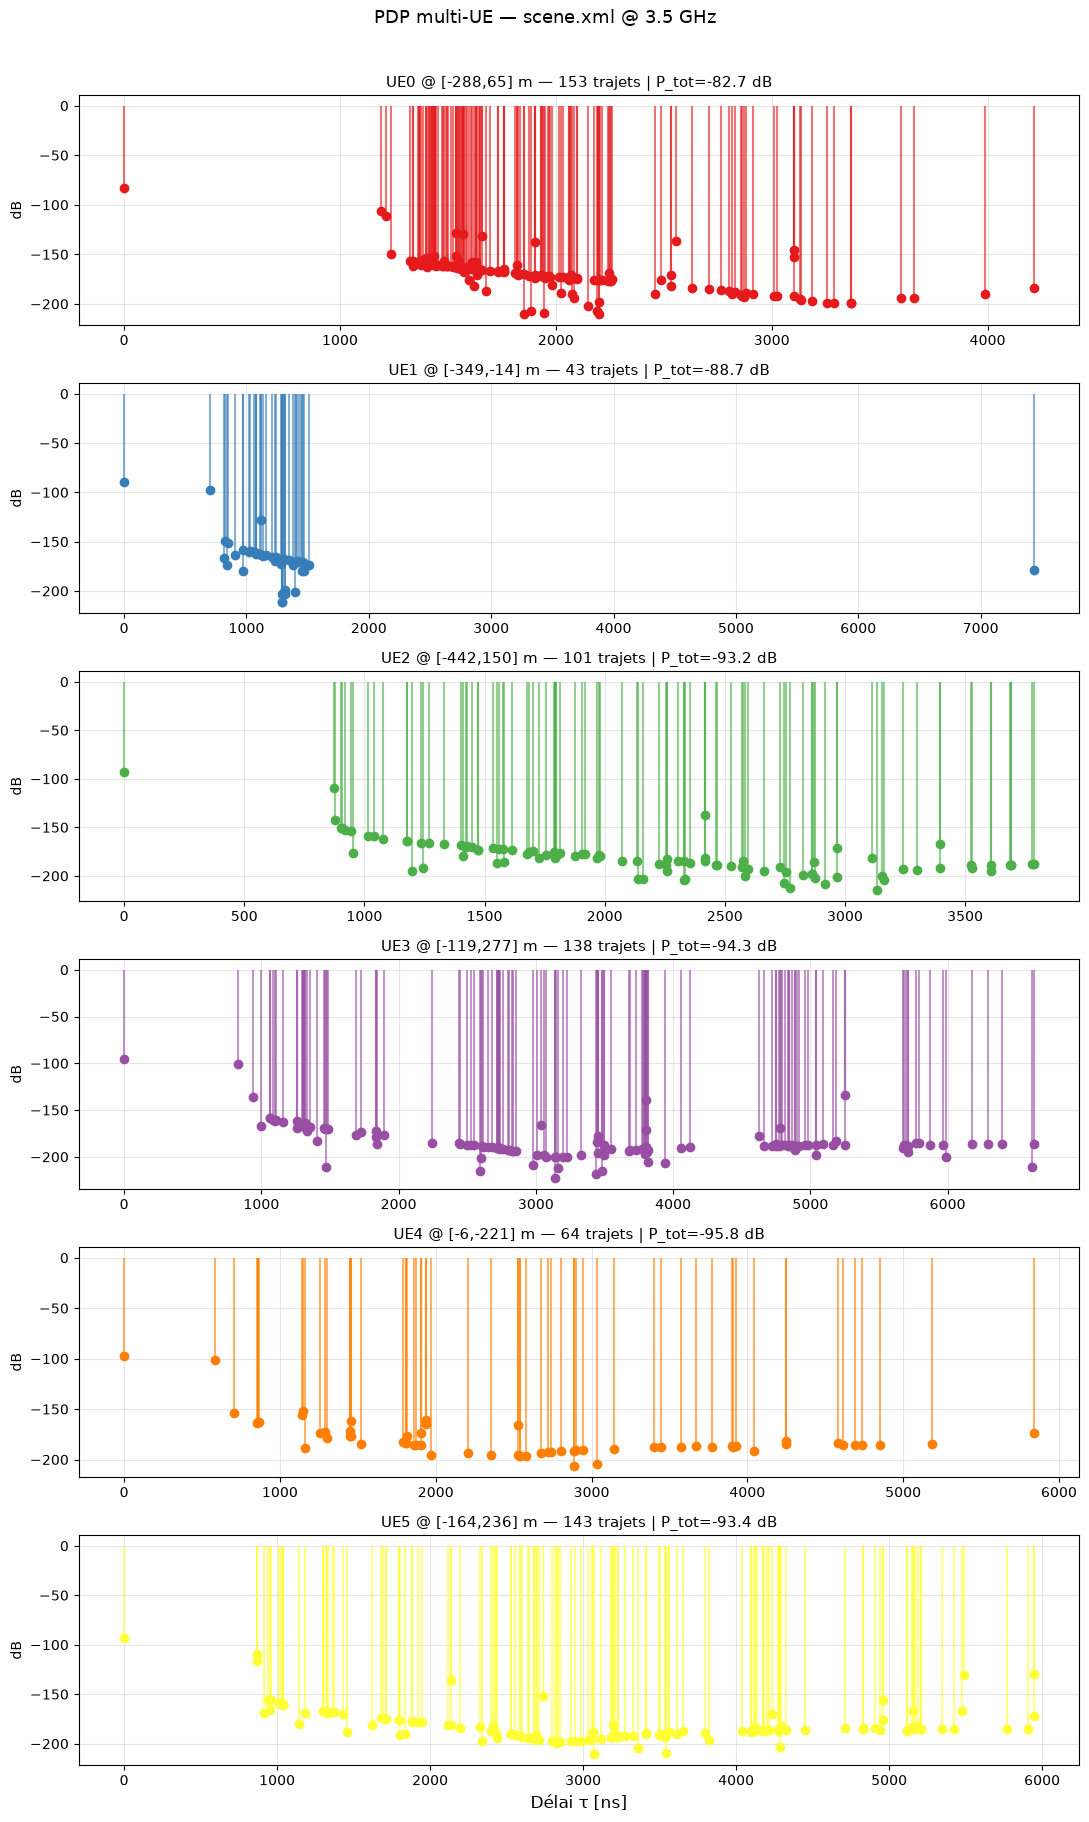
\includegraphics[width=0.85\textwidth]{figures/pdp_all_ue.png}
    \caption{Comparaison des PDP pour l'ensemble des six UE de la scène.}
    \label{fig:pdp_all}
\end{figure}

\begin{consoleout}
PDP multi-UE sauvegarde -> pdp_all_ue.png
\end{consoleout}

% ---------------------------------------------------------
\section{Carte de couverture radio (RadioMapSolver)}

Le \texttt{RadioMapSolver} calcule la puissance reçue sur une grille 2D --- utile pour valider la couverture de la BS et identifier les zones d'ombre.

\begin{lstlisting}
rm_solver = RadioMapSolver()

print("Calcul de la carte de couverture...")
t0 = time.time()

# RadioMapSolver 2.x : center/size/cell_size sont des params directs du call
# PAS de radio_map= ; pas de num_samples= (c'est samples_per_tx=)
radio_map = rm_solver(
    scene,
    center=[49.5, -38.5, 1.5],     # plan horizontal a 1.5 m (hauteur UE), centre sur la scene
    orientation=[0., 0., 0.],
    size=[2000., 2000.],              # 2000 m x 2000 m
    cell_size=[10., 10.],            # resolution 10 m
    max_depth=MAX_DEPTH,
    samples_per_tx=100000,
    diffuse_reflection=False,
    los=True,
    specular_reflection=True,
    diffraction=False,
    seed=42,
)

print(f"Carte calculee en {time.time()-t0:.2f} s")

# path_gain shape : [num_tx, cells_y, cells_x] -- avec plusieurs BS, on combine en
# "best server" (max lineaire par cellule) pour la carte de couverture globale.
path_gain_per_tx = np.array(radio_map.path_gain)   # [num_tx, cells_y, cells_x]
path_gain_combined = path_gain_per_tx.max(axis=0)  # meilleure BS par cellule
path_gain_db = 10 * np.log10(path_gain_combined + 1e-30)
print(f"Grille : {path_gain_db.shape[0]}x{path_gain_db.shape[1]} cellules ({path_gain_per_tx.shape[0]} BS combinees) | "
      f"Path gain : [{path_gain_db[path_gain_db>-200].min():.1f}, {path_gain_db.max():.1f}] dB")

fig, ax = plt.subplots(figsize=(8, 7))
im = ax.imshow(
    path_gain_db,
    origin="lower",
    cmap="jet",
    vmin=np.percentile(path_gain_db[path_gain_db > -200], 5),
    vmax=path_gain_db.max(),
)
plt.colorbar(im, ax=ax, label="Path Gain [dB]")
ax.set_title(
    f"Carte de couverture (best-server, {path_gain_per_tx.shape[0]} BS) "
    f"-- scene.xml @ {FREQUENCY_HZ/1e9:.1f} GHz\n"
    f"2000m x 2000m, resolution 10m"
)
ax.set_xlabel("X [cellules x 10 m]")
ax.set_ylabel("Y [cellules x 10 m]")
fig.tight_layout()
plt.savefig(WORKSPACE / "radio_map_riad.png", dpi=150, bbox_inches="tight")
plt.show()
print("Carte de couverture sauvegardee -> radio_map_riad.png")
\end{lstlisting}

\begin{figure}[H]
    \centering
    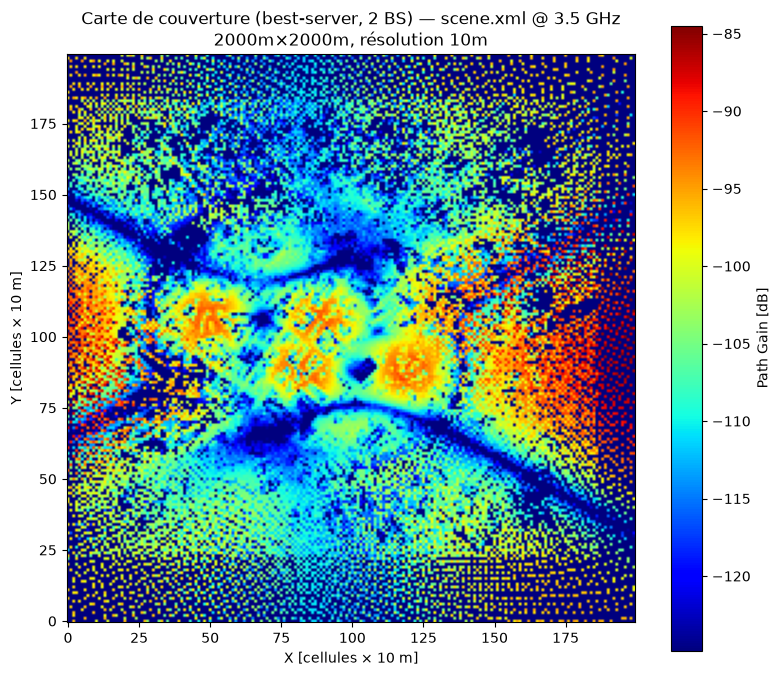
\includegraphics[width=0.75\textwidth]{figures/radio_map_riad.png}
    \caption{Carte de couverture radio (best-server, 2 BS combinées) sur la scène du secteur gouvernemental de Rabat, à \SI{3.5}{\giga\hertz}, résolution \SI{10}{\meter}.}
    \label{fig:radio_map}
\end{figure}

\begin{consoleout}
Calcul de la carte de couverture...
Carte calculee en 0.02 s
Grille : 200x200 cellules (2 BS combinees) | Path gain : [-187.7, -84.5] dB
Carte de couverture sauvegardee -> radio_map_riad.png
\end{consoleout}

\subsection*{Visualisation 3D de la carte de couverture}

Même principe que pour les trajets : \texttt{scene.render(camera=..., radio\_map=radio\_map)} en statique, \texttt{scene.preview(radio\_map=radio\_map)} en interactif live.

\begin{lstlisting}
# Camera dediee en vue de dessus, pour bien cadrer le plan de couverture 300x300 m
top_cam = Camera(
    position=[center_x, center_y, 2000],
    look_at=[center_x, center_y, 0.0],
)

if no_preview:
    scene.render(camera=top_cam, radio_map=radio_map, num_samples=256)
else:
    scene.preview(radio_map=radio_map)
\end{lstlisting}

\begin{figure}[H]
    \centering
    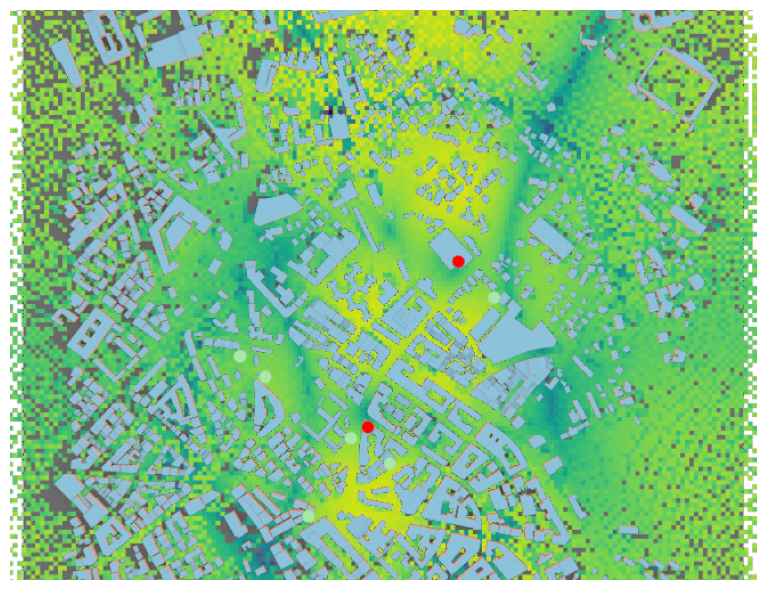
\includegraphics[width=0.75\textwidth]{figures/radio_map_3d_top.png}
    \caption{Rendu 3D de la carte de couverture radio, vue de dessus centrée sur la scène.}
    \label{fig:radio_map_3d}
\end{figure}

% ---------------------------------------------------------
\section{Paramètres ISAC --- Sorties pour la Phase 3}

Le ISAC (Integrated Sensing And Communications) exploite les paramètres de canal :
\begin{itemize}
    \item \textbf{Délais} $\tau_i$ $\to$ distance des cibles (range)
    \item \textbf{DoA} $\theta_i, \varphi_i$ $\to$ direction d'arrivée (localisation angulaire)
    \item \textbf{Doppler} $f_{\Delta,i}$ $\to$ vitesse radiale (si objets mobiles)
    \item \textbf{Puissances} $|a_i|^2$ $\to$ intensité de réflexion (matériau, distance)
\end{itemize}

\begin{lstlisting}
import warnings

isac_params = []

for rx_i in range(num_rx):
    tau_sel  = tau_cir[rx_i, 0, :]                         # [num_paths]
    a_sel    = a_complex[rx_i, :, 0, :, :, 0]              # [rx_ant, tx_ant, paths]
    power_all = np.abs(a_sel)**2
    power_mean = power_all.mean(axis=(0, 1))                # moyenne antennes -> [paths]

    valid    = tau_sel >= 0
    tau_v    = tau_sel[valid]
    power_v  = power_mean[valid]
    psum     = power_v.sum() + 1e-30

    # Delay spread (RMS)
    mean_tau = np.sum(power_v * tau_v) / psum
    rms_ds   = np.sqrt(np.sum(power_v * (tau_v - mean_tau)**2) / psum)

    # DoA : theta_t / phi_t si disponibles
    doa_theta, doa_phi = None, None
    with warnings.catch_warnings():
        warnings.simplefilter("ignore")
        try:
            doa_theta = np.array(paths.theta_t)[rx_i, 0, :][valid]
            doa_phi   = np.array(paths.phi_t)[rx_i, 0, :][valid]
        except Exception:
            pass

    rec = {
        "rx": f"ue{rx_i}",
        "tx": "bs0",
        "position_rx": RX_POSITIONS[rx_i],
        "num_valid_paths": int(valid.sum()),
        "delays_ns": (tau_v * 1e9).tolist(),
        "powers_db": (10 * np.log10(power_v + 1e-30)).tolist(),
        "total_power_db": float(10 * np.log10(psum)),
        "rms_delay_spread_ns": float(rms_ds * 1e9),
    }
    if doa_theta is not None:
        rec["doa_theta_deg"] = np.degrees(doa_theta).tolist()
        rec["doa_phi_deg"]   = np.degrees(doa_phi).tolist()

    isac_params.append(rec)
    print(f"UE{rx_i}: {rec['num_valid_paths']} trajets | "
          f"P_tot={rec['total_power_db']:.1f} dB | "
          f"DS_rms={rec['rms_delay_spread_ns']:.1f} ns")

print("\nParametres ISAC extraits.")
\end{lstlisting}

\begin{consoleout}
UE0: 153 trajets | P_tot=-82.7 dB | DS_rms=90.5 ns
UE1: 43 trajets | P_tot=-88.7 dB | DS_rms=243.4 ns
UE2: 101 trajets | P_tot=-93.2 dB | DS_rms=139.6 ns
UE3: 138 trajets | P_tot=-94.3 dB | DS_rms=349.8 ns
UE4: 64 trajets | P_tot=-95.8 dB | DS_rms=271.2 ns
UE5: 143 trajets | P_tot=-93.4 dB | DS_rms=190.1 ns

Parametres ISAC extraits.
\end{consoleout}

\begin{table}[H]
\centering
\begin{tabular}{lccc}
\toprule
\textbf{UE} & \textbf{Trajets valides} & \textbf{Puissance totale [dB]} & \textbf{Étalement RMS [ns]} \\
\midrule
UE0 & 153 & $-$82.7 & 90.5 \\
UE1 & 43  & $-$88.7 & 243.4 \\
UE2 & 101 & $-$93.2 & 139.6 \\
UE3 & 138 & $-$94.3 & 349.8 \\
UE4 & 64  & $-$95.8 & 271.2 \\
UE5 & 143 & $-$93.4 & 190.1 \\
\bottomrule
\end{tabular}
\caption{Paramètres ISAC extraits par liaison UE$\leftarrow$BS0}
\label{tab:isac}
\end{table}

% ---------------------------------------------------------
\section{Export Phase 2 \texorpdfstring{$\to$}{->} JSON (handoff vers Phase 3)}

\begin{lstlisting}
phase2_summary = {
    "project": "SDM-VA-ISAC",
    "phase": 2,
    "scene_xml": str(SCENE_XML),
    "mitsuba_variant": mi.variant(),
    "sionna_version": SIONNA_VERSION,
    "frequency_hz": float(FREQUENCY_HZ),
    "bandwidth_hz": float(BANDWIDTH_HZ),
    "max_depth": int(MAX_DEPTH),
    "tx_position": TX_POS,
    "rx_positions": RX_POSITIONS,
    "a_shape": list(a_complex.shape),
    "tau_shape": list(tau_cir.shape),
    "isac_per_link": isac_params,
    "validation": {
        "scene_loaded": True,
        "paths_found": int((tau_cir >= 0).sum()) > 0,
        "cir_extracted": True,
        "pdp_generated": True,
    }
}

out_path = WORKSPACE / "phase2_sionna_rt_summary.json"
with open(out_path, "w", encoding="utf-8") as f:
    json.dump(phase2_summary, f, indent=2)

print(f"Resume Phase 2 sauvegarde -> {out_path}")

v = phase2_summary["validation"]
print("\n=== VALIDATION PHASE 2 ===")
for k, ok in v.items():
    icon = "OK" if ok else "X"
    print(f"  {icon}  {k}")

if all(v.values()):
    print("\n>>> Phase 2 VALIDEE -- Pret pour la Phase 3 (fusion multimodale) <<<")
else:
    print("\n>>> Certains criteres non satisfaits -- verifier les erreurs ci-dessus")
\end{lstlisting}

\begin{consoleout}
Resume Phase 2 sauvegarde -> C:\Users\AdminFix\Desktop\PFA\phase2_sionna_rt_summary.json

=== VALIDATION PHASE 2 ===
  OK  scene_loaded
  OK  paths_found
  OK  cir_extracted
  OK  pdp_generated

>>> Phase 2 VALIDEE -- Pret pour la Phase 3 (fusion multimodale) <<<
\end{consoleout}

% ---------------------------------------------------------
\section{Conclusion}

Tous les critères de validation de la Phase 2 sont satisfaits : la scène XML se charge sans erreur, le \texttt{PathSolver} retourne des chemins exploitables (1174 trajets valides sur 2796), le CIR est extrait avec des dimensions cohérentes, les graphes PDP sont générés et le fichier \texttt{phase2\_sionna\_rt\_summary.json} est produit. Le pipeline Sionna RT sur la scène OSM/Blender est donc opérationnel et permet de passer à la Phase 3 du projet SDM-VA-ISAC (fusion multimodale).

\end{document}
